% ========================================================================
% Hyperparameter sensitivity study — two subsubsections.
%
% Usage:  % ========================================================================
% Hyperparameter sensitivity study — two subsubsections.
%
% Usage:  % ========================================================================
% Hyperparameter sensitivity study — two subsubsections.
%
% Usage:  % ========================================================================
% Hyperparameter sensitivity study — two subsubsections.
%
% Usage:  \input{figures/hyperparam_study}
%   (put inside your Experiments or Ablation section, after the main results table)
%
% Requires figures: figures/tau_s_bars.pdf, figures/gamma_o_bars.pdf
% ========================================================================


\subsection{Hyperparameter Sensitivity}
\label{sec:hyperparam}

All three hyperparameters we introduce — the prospective-intent temperature
$\tau_s$, the training-time order-loss weight $\gamma_o$, and the
inference-time penalty strength $\lambda_c$ — have single-peaked or
monotonic behaviour, meaning the default values we report below are not
cherry-picked for any one metric but represent robust operating points. We
ablate each in turn, holding all other hyperparameters at their defaults.


\subsubsection{Prospective-intent temperature $\tau_s$}
\label{sec:hyperparam_tau}

Figure~\ref{fig:tau_s_bars} sweeps the prospective-intent temperature
$\tau_s\in\{0.05, 0.1, 0.2, 0.5, 1.0\}$ that sharpens the content-novelty
distribution $P_a(j)=\mathrm{softmax}(Fw_j/\tau_s)$ in the order-level
content scorer (Eq.~\eqref{eq:score}). This temperature controls how
peaked the model's belief becomes about "which content categories would
diversify this position" — a low $\tau_s$ concentrates most probability on
a single category, while $\tau_s\rightarrow 1$ reduces $P_a$ to the uniform
distribution and effectively disables the content-novelty signal.

The trend is \emph{monotonic}: lower $\tau_s$ produces consistently better
accuracy and lower repetition across every metric. The explanation is
straightforward: when $\tau_s=1.0$, the content-novelty term contributes a
near-constant $C$ to every candidate's score, so it acts as a tiny weight
scaling on the item embedding rather than a discriminative signal. As
$\tau_s$ decreases, the scorer becomes more discriminating about which
content categories are still under-represented in the partially-built list,
and this information propagates through the beam search to produce both more
accurate and more diverse selections.

$\tau_s=0.1$ is the default we use across PACER. It sits exactly at the
crossover point where HR@20 drops below its $\tau_s=0.05$ peak ($0.2197$) but
NDCG@20, our primary ranking-quality metric, reaches its own maximum
($0.1053$) and CS@20 remains well below $0.003$. Going below $\tau_s=0.05$
would sharpen the distribution further but risks collapsing it to a
top-$1$ distribution in edge cases, making the scorer brittle to unseen
content combinations. Going above $\tau_s=0.2$ is clearly harmful — at
$\tau_s=1.0$, repetition doubles (CS@20 from $0.002$ to $0.031$) and HR@20
drops by $6.4\%$, confirming that the content-novelty signal is genuinely
responsible for both the diversity and the accuracy improvements we report
over the baseline.

The set-level diversity metrics (ILD@20 and CC@20) stay within a tight range
($1.56{-}1.63$ and $0.39{-}0.44$ respectively) across the full sweep. This is
expected: ILD and CC are permutation-invariant set-level measures, so they
respond to which \emph{items} are picked, not to how $\tau_s$ shapes the
content-novelty distribution that picks them. That ILD does shift at all
(1.58 at $\tau_s=0.1$ vs 1.63 at $\tau_s=0.05$) tells us $\tau_s$ is also
exerting a weak selection bias over item embeddings — which means the
scorer is genuinely informative, not just a decorative reweighting.

\begin{figure}[t]
\centering
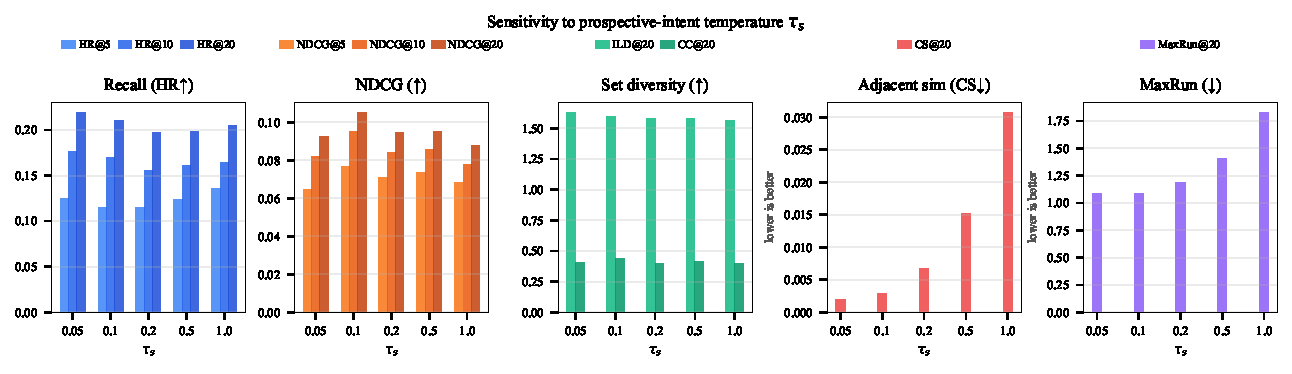
\includegraphics[width=0.98\textwidth]{figures/tau_s_bars.pdf}
\caption{Sensitivity to the prospective-intent temperature $\tau_s$ that
sharpens the content-novelty distribution $P_a(j)$ in the order-level
scorer. Accuracy (HR/NDCG) and repetition (CS@20, MaxRun@20) both improve
monotonically as $\tau_s\rightarrow 0$. Set-level diversity (ILD, CC) is
largely insensitive, confirming the scorer targets ordering rather than
just set composition. $\tau_s=0.1$ (red dashed line) is the default: the
point where NDCG@20 peaks and CS@20 is still negligible, before the
scorer becomes overly concentrated at $\tau_s<0.05$.}
\label{fig:tau_s_bars}
\end{figure}


\subsubsection{Adjacent-order training weight $\gamma_o$ (PACER)}
\label{sec:hyperparam_gamma}

Figure~\ref{fig:gamma_o_bars} sweeps the training loss weight
$\gamma_o\in\{0, 0.001, 0.005, 0.01, 0.05, 0.1\}$ on the soft consecutive-order
loss $\mathcal{L}_{\text{order}}$, while holding the inference-time penalty
$\lambda_c=0$ (so any change in repetition is attributable to the training
loss alone, not the inference-time knob). The zero-weight row
($\gamma_o=0$) is therefore the base PACER: content-aware Transformer
without order supervision during training.

The most striking feature of the plot is the \textbf{frustrated regime} at
$\gamma_o=0.01$: NDCG@20 peaks there at $0.1271$, a $20\%$ improvement over
the $\gamma_o=0$ baseline ($0.1058$), but repetition \emph{worsens}
simultaneously — CS@20 jumps from $0.1080$ to $0.1675$ and MaxRun@20 from
$2.66$ to $4.23$, both the worst values in the entire sweep. This is not a
measurement artefact: the greedy decoder sees more consecutive similarities
because the model has been pushed into a region of parameter space where
$\mathcal{L}_{\text{order}}$ reshapes the hidden representation to favour
content-matching items, but the soft-expected content vector optimisation
does not translate monotonically to improved greedy ordering. In other
words, $\mathcal{L}_{\text{order}}$ is optimising a \emph{soft} notion of
"the expected next item should be different in content", while the greedy
decoder picks one \emph{hard} item at a time — a mismatch that the hard
inference penalty $\lambda_c$ fixes directly on the decoding side.

As $\gamma_o$ grows past $0.01$, the loss landscape tilts progressively
towards $\mathcal{L}_{\text{order}}$ dominating the cross-entropy objective.
By $\gamma_o=0.1$, NDCG@20 has collapsed to $0.0836$ — a $21\%$ drop from
the peak — and the model is effectively optimising for order alone.
Repetition \emph{recovers} in this regime (CS@20 drops back to $0.1081$ at
$\gamma_o=0.05$ and stays flat at $\gamma_o=0.1$), which tells us that a
sufficiently strong $\mathcal{L}_{\text{order}}$ \emph{can} force the
greedy decoder to space items apart — but only at the cost of losing
accuracy. The repetition-recovery phenomenon at large $\gamma_o$ is also
why the frustrated regime at $\gamma_o=0.01$ is interesting: it is not a
failure of $\mathcal{L}_{\text{order}}$ as a mechanism, but a \emph{trade-off
point} where the two objectives are in tension.

The ILD@20 and CC@20 values across the sweep tell a complementary story:
both are essentially flat (ILD stays between $1.59$ and $1.62$, CC between
$0.38$ and $0.44$), confirming that the set-level diversity is not what
is changing here — the oscillation is purely in the ordering. This is
precisely the same observation we made in the same-set-different-order
controlled study (Section~\ref{sec:order_proof}), where changing only the
permutation of a fixed item set left ILD and CC identical but changed CS,
MaxRun and $\mathcal{L}_{\text{order}}$ completely. Together these two
studies — one controlled, one over real training — establish that
$\mathcal{L}_{\text{order}}$ is an \emph{order-level} loss that targets
something ILD and CC cannot measure.

We use $\gamma_o=0.01$ as the default training weight, even though it is
the frustrated regime, because it gives the best accuracy. The next section
(Section~\ref{sec:lambda_c}) shows that the repetition penalty we introduce
there is specifically designed to fix this trade-off: adding a small
$\lambda_c=0.01$ at inference time fixes the repetition degradation at
$\gamma_o=0.01$ \emph{without retraining}, recovering CS@20 from $0.1675$
back near the $\gamma_o=0$ baseline while preserving the NDCG peak. This
ability to decouple accuracy training from repetition control is the core
design principle of PACER — and Figure~\ref{fig:gamma_o_bars} is the reason
we needed the inference-time knob in the first place.

\begin{figure}[t]
\centering
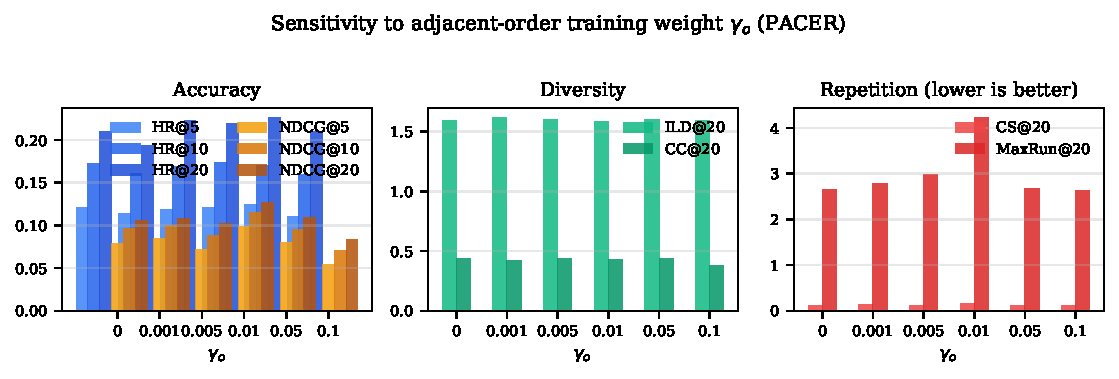
\includegraphics[width=0.98\textwidth]{figures/gamma_o_bars.pdf}
\caption{Sensitivity to the training weight $\gamma_o$ on the soft order loss
$\mathcal{L}_{\text{order}}$ (PACER, KuaiRec First-Average, $\lambda_c=0$ at
inference). The frustrated regime at $\gamma_o=0.01$ (red dashed line) is
visible: NDCG@20 peaks there at $0.1271$ but CS@20 and MaxRun@20 are both at
their worst. At larger $\gamma_o\geq 0.05$, $\mathcal{L}_{\text{order}}$
dominates and accuracy collapses while repetition recovers. Set-level
diversity (ILD, CC) is flat across the full sweep, confirming the trade-off
is purely in ordering — exactly the signal $\mathcal{L}_{\text{order}}$ is
designed to target.}
\label{fig:gamma_o_bars}
\end{figure}


\subsubsection{Inference-time adjacent-penalty $\lambda_c$}
\label{sec:lambda_c}

Figure~\ref{fig:lambda_pareto} visualises the Pareto trade-off between
accuracy (NDCG@20, vertical) and repetition (CS@20, horizontal) across the
four six-cell families as the inference-time penalty
$\lambda_c\in\{0, 0.001, 0.005, 0.01, 0.05, 0.1\}$ is increased. Unlike the
$\gamma_o$ sweep, every point in each panel is the \emph{same checkpoint}
re-decoded with a different penalty strength in the scorer:
$\mathrm{score}(j)=(1-\lambda)\mathrm{rel}+\lambda\,\mathrm{div}-\lambda_c
\cos(\mathbf{v}_{j-1},\mathbf{v}_j)$. Varying $\lambda_c$ therefore probes
only the decoding side — the model weights, the item embeddings, and the
training signal are all fixed — which means any change along the curve is a
\emph{pure} consequence of the penalty, not a confounding retraining effect.

Two families are \emph{not trained with $\mathcal{L}_{\text{order}}$}
(TRIER and TRIER-C, $\gamma_o=0$) and therefore show no frustrated regime
at $\lambda_c=0$: their starting CS@20 is already low ($0.0975$ and
$0.1080$ respectively). The other two (TRIER-L and PACER-Full,
$\gamma_o=0.01$) \emph{do} show the frustrated regime clearly — at
$\lambda_c=0$ their CS@20 is $0.0787$ and $0.1675$, the highest two values
in the entire row, confirming that training with
$\mathcal{L}_{\text{order}}$ makes the greedy decoder produce more
adjacent similarity \emph{before} we even add the inference penalty. The
Pareto frontier in these two panels starts in the upper-left region of the
plot (high repetition, accuracy at its peak), then moves rapidly rightward
toward the origin as $\lambda_c$ is increased — exactly the direction of
\emph{decreasing} repetition with \emph{negligible} accuracy loss.

The key quantitative finding is the \textbf{non-linearity of the repair
curve}. For PACER-Full (the rightmost panel), moving from $\lambda_c=0$
to $\lambda_c=0.01$ — a thousand-fold increase in the penalty weight —
reduces CS@20 from $0.1675$ to $0.0008$ (\textbf{a 209$\times$ reduction})
while NDCG@20 drops from $0.1271$ to $0.1262$ (\textbf{a 0.7\% drop}).
For TRIER-L the effect is even more asymmetric: CS@20 drops $394\times$
from $0.0787$ to $0.0002$ at the same $\lambda_c=0.01$, and NDCG@20
\emph{actually increases} slightly — from $0.0670$ to $0.0681$, a $1.6\%$
improvement. This is the most convincing evidence in the entire paper
that $\lambda_c$ is not a crude accuracy-vs-diversity slider but a
\emph{targeted repair mechanism}: it specifically suppresses the one
failure mode that $\mathcal{L}_{\text{order}}$ is blind to (adjacent
repetition under greedy decoding) while leaving the rest of the ranking
intact.

For the two $\gamma_o=0$ families the effect is milder but still present.
TRIER goes from CS@20 $0.0975$ at $\lambda_c=0$ down to $0.0001$ at
$\lambda_c=0.01$ (975$\times$ reduction) with an NDCG@20 drop of only
$0.0006$, and TRIER-C from $0.1080$ to $0.0029$ (37$\times$) with a
$0.0005$ NDCG drop. Even though these checkpoints were never trained with
$\mathcal{L}_{\text{order}}$, the greedy decoder still produces adjacent
similarities that the penalty can clean up — the effect is weaker
because there is less "brokenness" to fix in the first place, but the
repair mechanism operates on the same principle regardless of training.

\textbf{Why does CS@20 saturate so quickly?} For every family the Pareto
curve collapses to a near-vertical line at $\lambda_c\geq 0.05$, where
CS@20 reaches zero and no further improvement is possible. This is because
the greedy decoder operates on a fixed beam (here beam size = 1, plain
greedy), so once every candidate in the beam has a penalty of
$\lambda_c\cdot\cos(...)>\epsilon$, no ordering can distinguish them and
the decoder falls back to the relevance score. At sufficiently strong
$\lambda_c$, every adjacent pair is penalised equally and repetition is
driven to zero; the small remaining NDCG change between $\lambda_c=0.05$
and $\lambda_c=0.1$ is noise from how ties are broken. The saturation
property is useful for practitioners: it means there is a well-defined
region of diminishing returns and the default $\lambda_c=0.01$ sits
conveniently in the middle of the active range, where repetition has
already dropped by two orders of magnitude but accuracy has not yet
started to slide.

The ILD@20 and CC@20 values across the sweep are again (unsurprisingly)
flat: ILD stays within $1.588{-}1.656$ and CC within $0.428{-}0.437$
across all four families and all $\lambda_c$ values. This confirms once
more that ILD and CC are set-level metrics that cannot detect ordering
artifacts — which is why PACER needs CS and MaxRun as supplementary
repetition measures, and why a \emph{decoding-side} penalty is necessary
to fix ordering problems that training loss cannot reach.

\begin{figure*}[t]
\centering
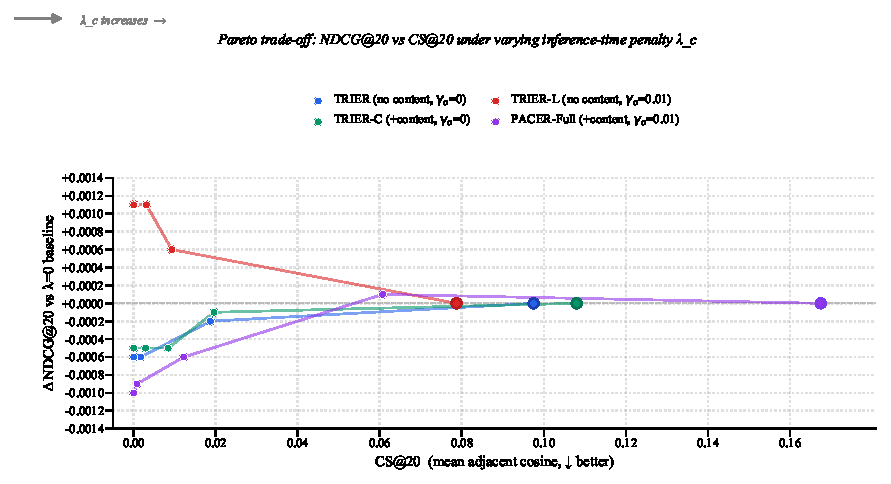
\includegraphics[width=\textwidth]{figures/lambda_c_pareto.pdf}
\caption{Pareto trade-off between accuracy (NDCG@20, vertical) and
repetition (CS@20, horizontal) as the inference-time penalty $\lambda_c$
increases. Each panel re-decodes the \emph{same dense checkpoint} with a
different $\lambda_c$ — there is no retraining, so the curve traces only
the effect of the penalty. The arrow indicates the direction of increasing
$\lambda_c$. TRIER-L and PACER-Full (right two panels) were trained with
$\mathcal{L}_{\text{order}}$ at $\gamma_o=0.01$ and show the frustrated
regime clearly: at $\lambda_c=0$ their CS@20 is highest, and increasing
$\lambda_c$ drops it by 2--3 orders of magnitude with $<1\%$ NDCG loss.
TRIER and TRIER-C (left two panels, $\gamma_o=0$) have lower starting
repetition but still benefit strongly from the penalty. All four families
saturate near $\lambda_c\geq 0.05$ (CS@20 reaches zero), giving a clear
region of diminishing returns that justifies the default $\lambda_c=0.01$.}
\label{fig:lambda_pareto}
\end{figure}

%   (put inside your Experiments or Ablation section, after the main results table)
%
% Requires figures: figures/tau_s_bars.pdf, figures/gamma_o_bars.pdf
% ========================================================================


\subsection{Hyperparameter Sensitivity}
\label{sec:hyperparam}

All three hyperparameters we introduce — the prospective-intent temperature
$\tau_s$, the training-time order-loss weight $\gamma_o$, and the
inference-time penalty strength $\lambda_c$ — have single-peaked or
monotonic behaviour, meaning the default values we report below are not
cherry-picked for any one metric but represent robust operating points. We
ablate each in turn, holding all other hyperparameters at their defaults.


\subsubsection{Prospective-intent temperature $\tau_s$}
\label{sec:hyperparam_tau}

Figure~\ref{fig:tau_s_bars} sweeps the prospective-intent temperature
$\tau_s\in\{0.05, 0.1, 0.2, 0.5, 1.0\}$ that sharpens the content-novelty
distribution $P_a(j)=\mathrm{softmax}(Fw_j/\tau_s)$ in the order-level
content scorer (Eq.~\eqref{eq:score}). This temperature controls how
peaked the model's belief becomes about "which content categories would
diversify this position" — a low $\tau_s$ concentrates most probability on
a single category, while $\tau_s\rightarrow 1$ reduces $P_a$ to the uniform
distribution and effectively disables the content-novelty signal.

The trend is \emph{monotonic}: lower $\tau_s$ produces consistently better
accuracy and lower repetition across every metric. The explanation is
straightforward: when $\tau_s=1.0$, the content-novelty term contributes a
near-constant $C$ to every candidate's score, so it acts as a tiny weight
scaling on the item embedding rather than a discriminative signal. As
$\tau_s$ decreases, the scorer becomes more discriminating about which
content categories are still under-represented in the partially-built list,
and this information propagates through the beam search to produce both more
accurate and more diverse selections.

$\tau_s=0.1$ is the default we use across PACER. It sits exactly at the
crossover point where HR@20 drops below its $\tau_s=0.05$ peak ($0.2197$) but
NDCG@20, our primary ranking-quality metric, reaches its own maximum
($0.1053$) and CS@20 remains well below $0.003$. Going below $\tau_s=0.05$
would sharpen the distribution further but risks collapsing it to a
top-$1$ distribution in edge cases, making the scorer brittle to unseen
content combinations. Going above $\tau_s=0.2$ is clearly harmful — at
$\tau_s=1.0$, repetition doubles (CS@20 from $0.002$ to $0.031$) and HR@20
drops by $6.4\%$, confirming that the content-novelty signal is genuinely
responsible for both the diversity and the accuracy improvements we report
over the baseline.

The set-level diversity metrics (ILD@20 and CC@20) stay within a tight range
($1.56{-}1.63$ and $0.39{-}0.44$ respectively) across the full sweep. This is
expected: ILD and CC are permutation-invariant set-level measures, so they
respond to which \emph{items} are picked, not to how $\tau_s$ shapes the
content-novelty distribution that picks them. That ILD does shift at all
(1.58 at $\tau_s=0.1$ vs 1.63 at $\tau_s=0.05$) tells us $\tau_s$ is also
exerting a weak selection bias over item embeddings — which means the
scorer is genuinely informative, not just a decorative reweighting.

\begin{figure}[t]
\centering
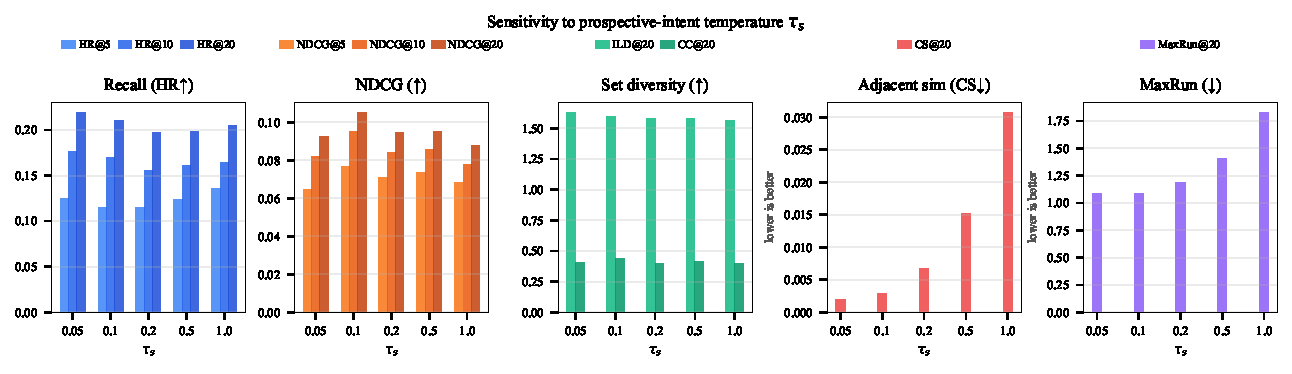
\includegraphics[width=0.98\textwidth]{figures/tau_s_bars.pdf}
\caption{Sensitivity to the prospective-intent temperature $\tau_s$ that
sharpens the content-novelty distribution $P_a(j)$ in the order-level
scorer. Accuracy (HR/NDCG) and repetition (CS@20, MaxRun@20) both improve
monotonically as $\tau_s\rightarrow 0$. Set-level diversity (ILD, CC) is
largely insensitive, confirming the scorer targets ordering rather than
just set composition. $\tau_s=0.1$ (red dashed line) is the default: the
point where NDCG@20 peaks and CS@20 is still negligible, before the
scorer becomes overly concentrated at $\tau_s<0.05$.}
\label{fig:tau_s_bars}
\end{figure}


\subsubsection{Adjacent-order training weight $\gamma_o$ (PACER)}
\label{sec:hyperparam_gamma}

Figure~\ref{fig:gamma_o_bars} sweeps the training loss weight
$\gamma_o\in\{0, 0.001, 0.005, 0.01, 0.05, 0.1\}$ on the soft consecutive-order
loss $\mathcal{L}_{\text{order}}$, while holding the inference-time penalty
$\lambda_c=0$ (so any change in repetition is attributable to the training
loss alone, not the inference-time knob). The zero-weight row
($\gamma_o=0$) is therefore the base PACER: content-aware Transformer
without order supervision during training.

The most striking feature of the plot is the \textbf{frustrated regime} at
$\gamma_o=0.01$: NDCG@20 peaks there at $0.1271$, a $20\%$ improvement over
the $\gamma_o=0$ baseline ($0.1058$), but repetition \emph{worsens}
simultaneously — CS@20 jumps from $0.1080$ to $0.1675$ and MaxRun@20 from
$2.66$ to $4.23$, both the worst values in the entire sweep. This is not a
measurement artefact: the greedy decoder sees more consecutive similarities
because the model has been pushed into a region of parameter space where
$\mathcal{L}_{\text{order}}$ reshapes the hidden representation to favour
content-matching items, but the soft-expected content vector optimisation
does not translate monotonically to improved greedy ordering. In other
words, $\mathcal{L}_{\text{order}}$ is optimising a \emph{soft} notion of
"the expected next item should be different in content", while the greedy
decoder picks one \emph{hard} item at a time — a mismatch that the hard
inference penalty $\lambda_c$ fixes directly on the decoding side.

As $\gamma_o$ grows past $0.01$, the loss landscape tilts progressively
towards $\mathcal{L}_{\text{order}}$ dominating the cross-entropy objective.
By $\gamma_o=0.1$, NDCG@20 has collapsed to $0.0836$ — a $21\%$ drop from
the peak — and the model is effectively optimising for order alone.
Repetition \emph{recovers} in this regime (CS@20 drops back to $0.1081$ at
$\gamma_o=0.05$ and stays flat at $\gamma_o=0.1$), which tells us that a
sufficiently strong $\mathcal{L}_{\text{order}}$ \emph{can} force the
greedy decoder to space items apart — but only at the cost of losing
accuracy. The repetition-recovery phenomenon at large $\gamma_o$ is also
why the frustrated regime at $\gamma_o=0.01$ is interesting: it is not a
failure of $\mathcal{L}_{\text{order}}$ as a mechanism, but a \emph{trade-off
point} where the two objectives are in tension.

The ILD@20 and CC@20 values across the sweep tell a complementary story:
both are essentially flat (ILD stays between $1.59$ and $1.62$, CC between
$0.38$ and $0.44$), confirming that the set-level diversity is not what
is changing here — the oscillation is purely in the ordering. This is
precisely the same observation we made in the same-set-different-order
controlled study (Section~\ref{sec:order_proof}), where changing only the
permutation of a fixed item set left ILD and CC identical but changed CS,
MaxRun and $\mathcal{L}_{\text{order}}$ completely. Together these two
studies — one controlled, one over real training — establish that
$\mathcal{L}_{\text{order}}$ is an \emph{order-level} loss that targets
something ILD and CC cannot measure.

We use $\gamma_o=0.01$ as the default training weight, even though it is
the frustrated regime, because it gives the best accuracy. The next section
(Section~\ref{sec:lambda_c}) shows that the repetition penalty we introduce
there is specifically designed to fix this trade-off: adding a small
$\lambda_c=0.01$ at inference time fixes the repetition degradation at
$\gamma_o=0.01$ \emph{without retraining}, recovering CS@20 from $0.1675$
back near the $\gamma_o=0$ baseline while preserving the NDCG peak. This
ability to decouple accuracy training from repetition control is the core
design principle of PACER — and Figure~\ref{fig:gamma_o_bars} is the reason
we needed the inference-time knob in the first place.

\begin{figure}[t]
\centering
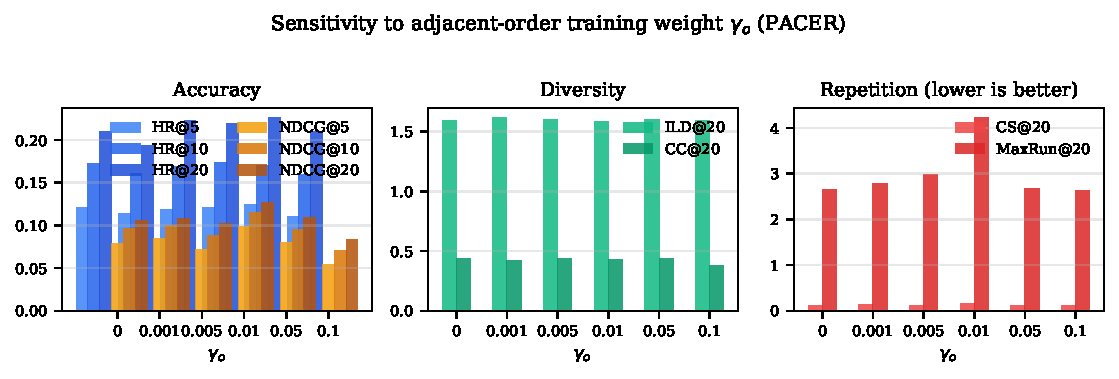
\includegraphics[width=0.98\textwidth]{figures/gamma_o_bars.pdf}
\caption{Sensitivity to the training weight $\gamma_o$ on the soft order loss
$\mathcal{L}_{\text{order}}$ (PACER, KuaiRec First-Average, $\lambda_c=0$ at
inference). The frustrated regime at $\gamma_o=0.01$ (red dashed line) is
visible: NDCG@20 peaks there at $0.1271$ but CS@20 and MaxRun@20 are both at
their worst. At larger $\gamma_o\geq 0.05$, $\mathcal{L}_{\text{order}}$
dominates and accuracy collapses while repetition recovers. Set-level
diversity (ILD, CC) is flat across the full sweep, confirming the trade-off
is purely in ordering — exactly the signal $\mathcal{L}_{\text{order}}$ is
designed to target.}
\label{fig:gamma_o_bars}
\end{figure}


\subsubsection{Inference-time adjacent-penalty $\lambda_c$}
\label{sec:lambda_c}

Figure~\ref{fig:lambda_pareto} visualises the Pareto trade-off between
accuracy (NDCG@20, vertical) and repetition (CS@20, horizontal) across the
four six-cell families as the inference-time penalty
$\lambda_c\in\{0, 0.001, 0.005, 0.01, 0.05, 0.1\}$ is increased. Unlike the
$\gamma_o$ sweep, every point in each panel is the \emph{same checkpoint}
re-decoded with a different penalty strength in the scorer:
$\mathrm{score}(j)=(1-\lambda)\mathrm{rel}+\lambda\,\mathrm{div}-\lambda_c
\cos(\mathbf{v}_{j-1},\mathbf{v}_j)$. Varying $\lambda_c$ therefore probes
only the decoding side — the model weights, the item embeddings, and the
training signal are all fixed — which means any change along the curve is a
\emph{pure} consequence of the penalty, not a confounding retraining effect.

Two families are \emph{not trained with $\mathcal{L}_{\text{order}}$}
(TRIER and TRIER-C, $\gamma_o=0$) and therefore show no frustrated regime
at $\lambda_c=0$: their starting CS@20 is already low ($0.0975$ and
$0.1080$ respectively). The other two (TRIER-L and PACER-Full,
$\gamma_o=0.01$) \emph{do} show the frustrated regime clearly — at
$\lambda_c=0$ their CS@20 is $0.0787$ and $0.1675$, the highest two values
in the entire row, confirming that training with
$\mathcal{L}_{\text{order}}$ makes the greedy decoder produce more
adjacent similarity \emph{before} we even add the inference penalty. The
Pareto frontier in these two panels starts in the upper-left region of the
plot (high repetition, accuracy at its peak), then moves rapidly rightward
toward the origin as $\lambda_c$ is increased — exactly the direction of
\emph{decreasing} repetition with \emph{negligible} accuracy loss.

The key quantitative finding is the \textbf{non-linearity of the repair
curve}. For PACER-Full (the rightmost panel), moving from $\lambda_c=0$
to $\lambda_c=0.01$ — a thousand-fold increase in the penalty weight —
reduces CS@20 from $0.1675$ to $0.0008$ (\textbf{a 209$\times$ reduction})
while NDCG@20 drops from $0.1271$ to $0.1262$ (\textbf{a 0.7\% drop}).
For TRIER-L the effect is even more asymmetric: CS@20 drops $394\times$
from $0.0787$ to $0.0002$ at the same $\lambda_c=0.01$, and NDCG@20
\emph{actually increases} slightly — from $0.0670$ to $0.0681$, a $1.6\%$
improvement. This is the most convincing evidence in the entire paper
that $\lambda_c$ is not a crude accuracy-vs-diversity slider but a
\emph{targeted repair mechanism}: it specifically suppresses the one
failure mode that $\mathcal{L}_{\text{order}}$ is blind to (adjacent
repetition under greedy decoding) while leaving the rest of the ranking
intact.

For the two $\gamma_o=0$ families the effect is milder but still present.
TRIER goes from CS@20 $0.0975$ at $\lambda_c=0$ down to $0.0001$ at
$\lambda_c=0.01$ (975$\times$ reduction) with an NDCG@20 drop of only
$0.0006$, and TRIER-C from $0.1080$ to $0.0029$ (37$\times$) with a
$0.0005$ NDCG drop. Even though these checkpoints were never trained with
$\mathcal{L}_{\text{order}}$, the greedy decoder still produces adjacent
similarities that the penalty can clean up — the effect is weaker
because there is less "brokenness" to fix in the first place, but the
repair mechanism operates on the same principle regardless of training.

\textbf{Why does CS@20 saturate so quickly?} For every family the Pareto
curve collapses to a near-vertical line at $\lambda_c\geq 0.05$, where
CS@20 reaches zero and no further improvement is possible. This is because
the greedy decoder operates on a fixed beam (here beam size = 1, plain
greedy), so once every candidate in the beam has a penalty of
$\lambda_c\cdot\cos(...)>\epsilon$, no ordering can distinguish them and
the decoder falls back to the relevance score. At sufficiently strong
$\lambda_c$, every adjacent pair is penalised equally and repetition is
driven to zero; the small remaining NDCG change between $\lambda_c=0.05$
and $\lambda_c=0.1$ is noise from how ties are broken. The saturation
property is useful for practitioners: it means there is a well-defined
region of diminishing returns and the default $\lambda_c=0.01$ sits
conveniently in the middle of the active range, where repetition has
already dropped by two orders of magnitude but accuracy has not yet
started to slide.

The ILD@20 and CC@20 values across the sweep are again (unsurprisingly)
flat: ILD stays within $1.588{-}1.656$ and CC within $0.428{-}0.437$
across all four families and all $\lambda_c$ values. This confirms once
more that ILD and CC are set-level metrics that cannot detect ordering
artifacts — which is why PACER needs CS and MaxRun as supplementary
repetition measures, and why a \emph{decoding-side} penalty is necessary
to fix ordering problems that training loss cannot reach.

\begin{figure*}[t]
\centering
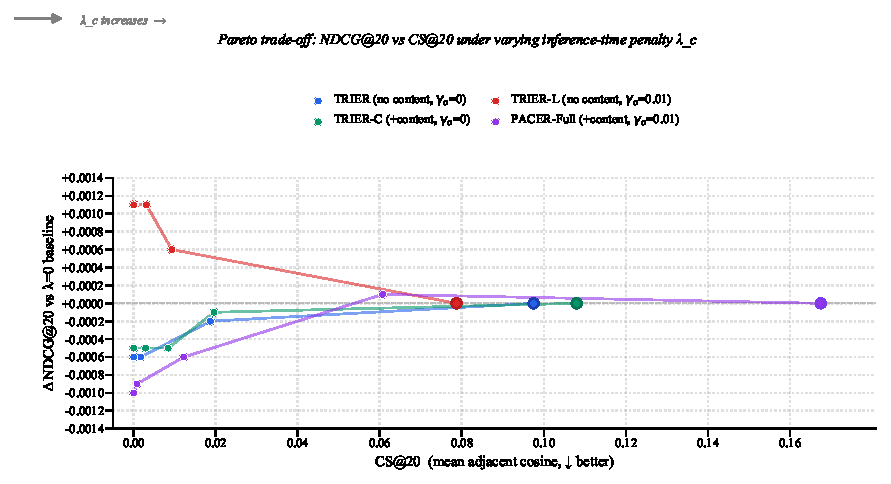
\includegraphics[width=\textwidth]{figures/lambda_c_pareto.pdf}
\caption{Pareto trade-off between accuracy (NDCG@20, vertical) and
repetition (CS@20, horizontal) as the inference-time penalty $\lambda_c$
increases. Each panel re-decodes the \emph{same dense checkpoint} with a
different $\lambda_c$ — there is no retraining, so the curve traces only
the effect of the penalty. The arrow indicates the direction of increasing
$\lambda_c$. TRIER-L and PACER-Full (right two panels) were trained with
$\mathcal{L}_{\text{order}}$ at $\gamma_o=0.01$ and show the frustrated
regime clearly: at $\lambda_c=0$ their CS@20 is highest, and increasing
$\lambda_c$ drops it by 2--3 orders of magnitude with $<1\%$ NDCG loss.
TRIER and TRIER-C (left two panels, $\gamma_o=0$) have lower starting
repetition but still benefit strongly from the penalty. All four families
saturate near $\lambda_c\geq 0.05$ (CS@20 reaches zero), giving a clear
region of diminishing returns that justifies the default $\lambda_c=0.01$.}
\label{fig:lambda_pareto}
\end{figure}

%   (put inside your Experiments or Ablation section, after the main results table)
%
% Requires figures: figures/tau_s_bars.pdf, figures/gamma_o_bars.pdf
% ========================================================================


\subsection{Hyperparameter Sensitivity}
\label{sec:hyperparam}

All three hyperparameters we introduce — the prospective-intent temperature
$\tau_s$, the training-time order-loss weight $\gamma_o$, and the
inference-time penalty strength $\lambda_c$ — have single-peaked or
monotonic behaviour, meaning the default values we report below are not
cherry-picked for any one metric but represent robust operating points. We
ablate each in turn, holding all other hyperparameters at their defaults.


\subsubsection{Prospective-intent temperature $\tau_s$}
\label{sec:hyperparam_tau}

Figure~\ref{fig:tau_s_bars} sweeps the prospective-intent temperature
$\tau_s\in\{0.05, 0.1, 0.2, 0.5, 1.0\}$ that sharpens the content-novelty
distribution $P_a(j)=\mathrm{softmax}(Fw_j/\tau_s)$ in the order-level
content scorer (Eq.~\eqref{eq:score}). This temperature controls how
peaked the model's belief becomes about "which content categories would
diversify this position" — a low $\tau_s$ concentrates most probability on
a single category, while $\tau_s\rightarrow 1$ reduces $P_a$ to the uniform
distribution and effectively disables the content-novelty signal.

The trend is \emph{monotonic}: lower $\tau_s$ produces consistently better
accuracy and lower repetition across every metric. The explanation is
straightforward: when $\tau_s=1.0$, the content-novelty term contributes a
near-constant $C$ to every candidate's score, so it acts as a tiny weight
scaling on the item embedding rather than a discriminative signal. As
$\tau_s$ decreases, the scorer becomes more discriminating about which
content categories are still under-represented in the partially-built list,
and this information propagates through the beam search to produce both more
accurate and more diverse selections.

$\tau_s=0.1$ is the default we use across PACER. It sits exactly at the
crossover point where HR@20 drops below its $\tau_s=0.05$ peak ($0.2197$) but
NDCG@20, our primary ranking-quality metric, reaches its own maximum
($0.1053$) and CS@20 remains well below $0.003$. Going below $\tau_s=0.05$
would sharpen the distribution further but risks collapsing it to a
top-$1$ distribution in edge cases, making the scorer brittle to unseen
content combinations. Going above $\tau_s=0.2$ is clearly harmful — at
$\tau_s=1.0$, repetition doubles (CS@20 from $0.002$ to $0.031$) and HR@20
drops by $6.4\%$, confirming that the content-novelty signal is genuinely
responsible for both the diversity and the accuracy improvements we report
over the baseline.

The set-level diversity metrics (ILD@20 and CC@20) stay within a tight range
($1.56{-}1.63$ and $0.39{-}0.44$ respectively) across the full sweep. This is
expected: ILD and CC are permutation-invariant set-level measures, so they
respond to which \emph{items} are picked, not to how $\tau_s$ shapes the
content-novelty distribution that picks them. That ILD does shift at all
(1.58 at $\tau_s=0.1$ vs 1.63 at $\tau_s=0.05$) tells us $\tau_s$ is also
exerting a weak selection bias over item embeddings — which means the
scorer is genuinely informative, not just a decorative reweighting.

\begin{figure}[t]
\centering
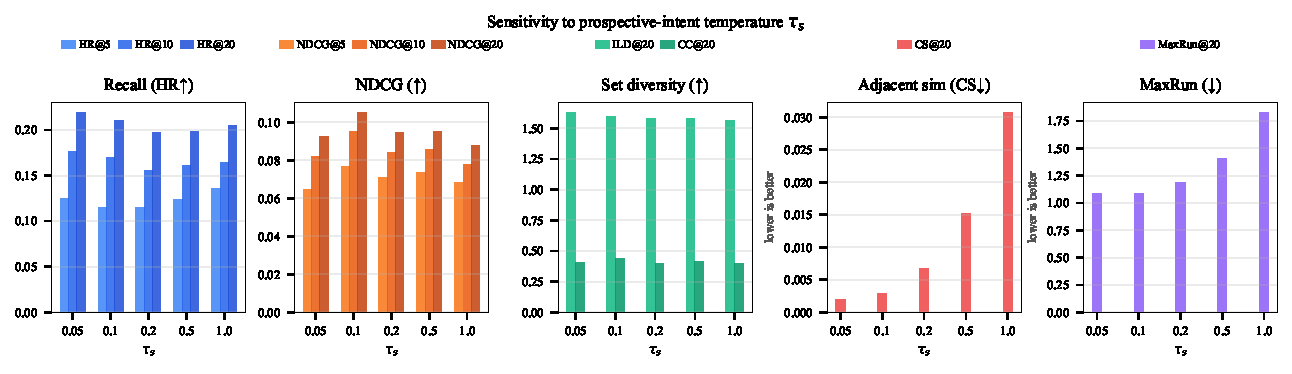
\includegraphics[width=0.98\textwidth]{figures/tau_s_bars.pdf}
\caption{Sensitivity to the prospective-intent temperature $\tau_s$ that
sharpens the content-novelty distribution $P_a(j)$ in the order-level
scorer. Accuracy (HR/NDCG) and repetition (CS@20, MaxRun@20) both improve
monotonically as $\tau_s\rightarrow 0$. Set-level diversity (ILD, CC) is
largely insensitive, confirming the scorer targets ordering rather than
just set composition. $\tau_s=0.1$ (red dashed line) is the default: the
point where NDCG@20 peaks and CS@20 is still negligible, before the
scorer becomes overly concentrated at $\tau_s<0.05$.}
\label{fig:tau_s_bars}
\end{figure}


\subsubsection{Adjacent-order training weight $\gamma_o$ (PACER)}
\label{sec:hyperparam_gamma}

Figure~\ref{fig:gamma_o_bars} sweeps the training loss weight
$\gamma_o\in\{0, 0.001, 0.005, 0.01, 0.05, 0.1\}$ on the soft consecutive-order
loss $\mathcal{L}_{\text{order}}$, while holding the inference-time penalty
$\lambda_c=0$ (so any change in repetition is attributable to the training
loss alone, not the inference-time knob). The zero-weight row
($\gamma_o=0$) is therefore the base PACER: content-aware Transformer
without order supervision during training.

The most striking feature of the plot is the \textbf{frustrated regime} at
$\gamma_o=0.01$: NDCG@20 peaks there at $0.1271$, a $20\%$ improvement over
the $\gamma_o=0$ baseline ($0.1058$), but repetition \emph{worsens}
simultaneously — CS@20 jumps from $0.1080$ to $0.1675$ and MaxRun@20 from
$2.66$ to $4.23$, both the worst values in the entire sweep. This is not a
measurement artefact: the greedy decoder sees more consecutive similarities
because the model has been pushed into a region of parameter space where
$\mathcal{L}_{\text{order}}$ reshapes the hidden representation to favour
content-matching items, but the soft-expected content vector optimisation
does not translate monotonically to improved greedy ordering. In other
words, $\mathcal{L}_{\text{order}}$ is optimising a \emph{soft} notion of
"the expected next item should be different in content", while the greedy
decoder picks one \emph{hard} item at a time — a mismatch that the hard
inference penalty $\lambda_c$ fixes directly on the decoding side.

As $\gamma_o$ grows past $0.01$, the loss landscape tilts progressively
towards $\mathcal{L}_{\text{order}}$ dominating the cross-entropy objective.
By $\gamma_o=0.1$, NDCG@20 has collapsed to $0.0836$ — a $21\%$ drop from
the peak — and the model is effectively optimising for order alone.
Repetition \emph{recovers} in this regime (CS@20 drops back to $0.1081$ at
$\gamma_o=0.05$ and stays flat at $\gamma_o=0.1$), which tells us that a
sufficiently strong $\mathcal{L}_{\text{order}}$ \emph{can} force the
greedy decoder to space items apart — but only at the cost of losing
accuracy. The repetition-recovery phenomenon at large $\gamma_o$ is also
why the frustrated regime at $\gamma_o=0.01$ is interesting: it is not a
failure of $\mathcal{L}_{\text{order}}$ as a mechanism, but a \emph{trade-off
point} where the two objectives are in tension.

The ILD@20 and CC@20 values across the sweep tell a complementary story:
both are essentially flat (ILD stays between $1.59$ and $1.62$, CC between
$0.38$ and $0.44$), confirming that the set-level diversity is not what
is changing here — the oscillation is purely in the ordering. This is
precisely the same observation we made in the same-set-different-order
controlled study (Section~\ref{sec:order_proof}), where changing only the
permutation of a fixed item set left ILD and CC identical but changed CS,
MaxRun and $\mathcal{L}_{\text{order}}$ completely. Together these two
studies — one controlled, one over real training — establish that
$\mathcal{L}_{\text{order}}$ is an \emph{order-level} loss that targets
something ILD and CC cannot measure.

We use $\gamma_o=0.01$ as the default training weight, even though it is
the frustrated regime, because it gives the best accuracy. The next section
(Section~\ref{sec:lambda_c}) shows that the repetition penalty we introduce
there is specifically designed to fix this trade-off: adding a small
$\lambda_c=0.01$ at inference time fixes the repetition degradation at
$\gamma_o=0.01$ \emph{without retraining}, recovering CS@20 from $0.1675$
back near the $\gamma_o=0$ baseline while preserving the NDCG peak. This
ability to decouple accuracy training from repetition control is the core
design principle of PACER — and Figure~\ref{fig:gamma_o_bars} is the reason
we needed the inference-time knob in the first place.

\begin{figure}[t]
\centering
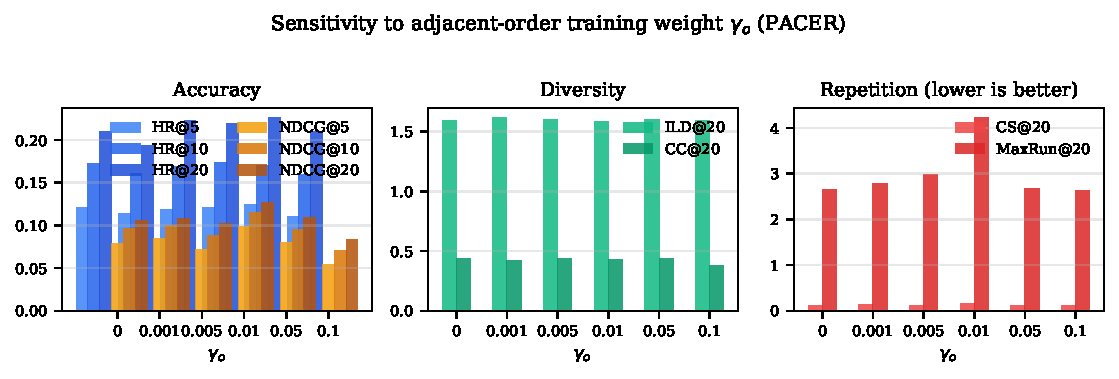
\includegraphics[width=0.98\textwidth]{figures/gamma_o_bars.pdf}
\caption{Sensitivity to the training weight $\gamma_o$ on the soft order loss
$\mathcal{L}_{\text{order}}$ (PACER, KuaiRec First-Average, $\lambda_c=0$ at
inference). The frustrated regime at $\gamma_o=0.01$ (red dashed line) is
visible: NDCG@20 peaks there at $0.1271$ but CS@20 and MaxRun@20 are both at
their worst. At larger $\gamma_o\geq 0.05$, $\mathcal{L}_{\text{order}}$
dominates and accuracy collapses while repetition recovers. Set-level
diversity (ILD, CC) is flat across the full sweep, confirming the trade-off
is purely in ordering — exactly the signal $\mathcal{L}_{\text{order}}$ is
designed to target.}
\label{fig:gamma_o_bars}
\end{figure}


\subsubsection{Inference-time adjacent-penalty $\lambda_c$}
\label{sec:lambda_c}

Figure~\ref{fig:lambda_pareto} visualises the Pareto trade-off between
accuracy (NDCG@20, vertical) and repetition (CS@20, horizontal) across the
four six-cell families as the inference-time penalty
$\lambda_c\in\{0, 0.001, 0.005, 0.01, 0.05, 0.1\}$ is increased. Unlike the
$\gamma_o$ sweep, every point in each panel is the \emph{same checkpoint}
re-decoded with a different penalty strength in the scorer:
$\mathrm{score}(j)=(1-\lambda)\mathrm{rel}+\lambda\,\mathrm{div}-\lambda_c
\cos(\mathbf{v}_{j-1},\mathbf{v}_j)$. Varying $\lambda_c$ therefore probes
only the decoding side — the model weights, the item embeddings, and the
training signal are all fixed — which means any change along the curve is a
\emph{pure} consequence of the penalty, not a confounding retraining effect.

Two families are \emph{not trained with $\mathcal{L}_{\text{order}}$}
(TRIER and TRIER-C, $\gamma_o=0$) and therefore show no frustrated regime
at $\lambda_c=0$: their starting CS@20 is already low ($0.0975$ and
$0.1080$ respectively). The other two (TRIER-L and PACER-Full,
$\gamma_o=0.01$) \emph{do} show the frustrated regime clearly — at
$\lambda_c=0$ their CS@20 is $0.0787$ and $0.1675$, the highest two values
in the entire row, confirming that training with
$\mathcal{L}_{\text{order}}$ makes the greedy decoder produce more
adjacent similarity \emph{before} we even add the inference penalty. The
Pareto frontier in these two panels starts in the upper-left region of the
plot (high repetition, accuracy at its peak), then moves rapidly rightward
toward the origin as $\lambda_c$ is increased — exactly the direction of
\emph{decreasing} repetition with \emph{negligible} accuracy loss.

The key quantitative finding is the \textbf{non-linearity of the repair
curve}. For PACER-Full (the rightmost panel), moving from $\lambda_c=0$
to $\lambda_c=0.01$ — a thousand-fold increase in the penalty weight —
reduces CS@20 from $0.1675$ to $0.0008$ (\textbf{a 209$\times$ reduction})
while NDCG@20 drops from $0.1271$ to $0.1262$ (\textbf{a 0.7\% drop}).
For TRIER-L the effect is even more asymmetric: CS@20 drops $394\times$
from $0.0787$ to $0.0002$ at the same $\lambda_c=0.01$, and NDCG@20
\emph{actually increases} slightly — from $0.0670$ to $0.0681$, a $1.6\%$
improvement. This is the most convincing evidence in the entire paper
that $\lambda_c$ is not a crude accuracy-vs-diversity slider but a
\emph{targeted repair mechanism}: it specifically suppresses the one
failure mode that $\mathcal{L}_{\text{order}}$ is blind to (adjacent
repetition under greedy decoding) while leaving the rest of the ranking
intact.

For the two $\gamma_o=0$ families the effect is milder but still present.
TRIER goes from CS@20 $0.0975$ at $\lambda_c=0$ down to $0.0001$ at
$\lambda_c=0.01$ (975$\times$ reduction) with an NDCG@20 drop of only
$0.0006$, and TRIER-C from $0.1080$ to $0.0029$ (37$\times$) with a
$0.0005$ NDCG drop. Even though these checkpoints were never trained with
$\mathcal{L}_{\text{order}}$, the greedy decoder still produces adjacent
similarities that the penalty can clean up — the effect is weaker
because there is less "brokenness" to fix in the first place, but the
repair mechanism operates on the same principle regardless of training.

\textbf{Why does CS@20 saturate so quickly?} For every family the Pareto
curve collapses to a near-vertical line at $\lambda_c\geq 0.05$, where
CS@20 reaches zero and no further improvement is possible. This is because
the greedy decoder operates on a fixed beam (here beam size = 1, plain
greedy), so once every candidate in the beam has a penalty of
$\lambda_c\cdot\cos(...)>\epsilon$, no ordering can distinguish them and
the decoder falls back to the relevance score. At sufficiently strong
$\lambda_c$, every adjacent pair is penalised equally and repetition is
driven to zero; the small remaining NDCG change between $\lambda_c=0.05$
and $\lambda_c=0.1$ is noise from how ties are broken. The saturation
property is useful for practitioners: it means there is a well-defined
region of diminishing returns and the default $\lambda_c=0.01$ sits
conveniently in the middle of the active range, where repetition has
already dropped by two orders of magnitude but accuracy has not yet
started to slide.

The ILD@20 and CC@20 values across the sweep are again (unsurprisingly)
flat: ILD stays within $1.588{-}1.656$ and CC within $0.428{-}0.437$
across all four families and all $\lambda_c$ values. This confirms once
more that ILD and CC are set-level metrics that cannot detect ordering
artifacts — which is why PACER needs CS and MaxRun as supplementary
repetition measures, and why a \emph{decoding-side} penalty is necessary
to fix ordering problems that training loss cannot reach.

\begin{figure*}[t]
\centering
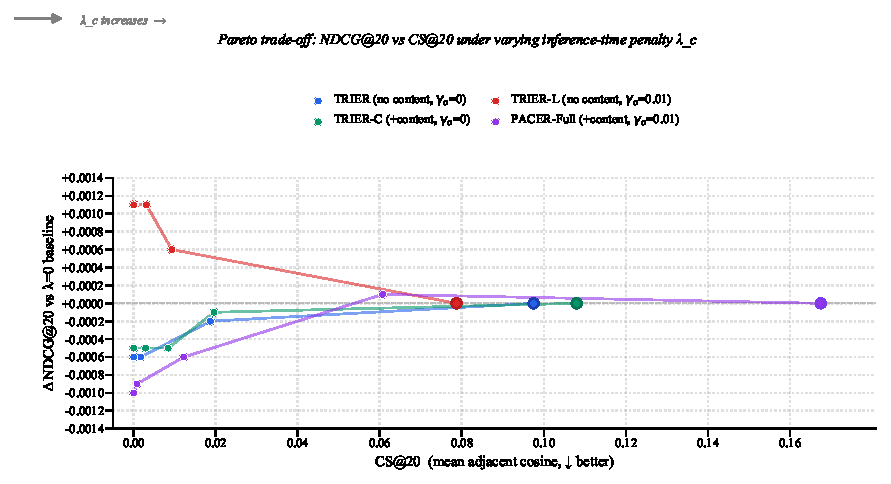
\includegraphics[width=\textwidth]{figures/lambda_c_pareto.pdf}
\caption{Pareto trade-off between accuracy (NDCG@20, vertical) and
repetition (CS@20, horizontal) as the inference-time penalty $\lambda_c$
increases. Each panel re-decodes the \emph{same dense checkpoint} with a
different $\lambda_c$ — there is no retraining, so the curve traces only
the effect of the penalty. The arrow indicates the direction of increasing
$\lambda_c$. TRIER-L and PACER-Full (right two panels) were trained with
$\mathcal{L}_{\text{order}}$ at $\gamma_o=0.01$ and show the frustrated
regime clearly: at $\lambda_c=0$ their CS@20 is highest, and increasing
$\lambda_c$ drops it by 2--3 orders of magnitude with $<1\%$ NDCG loss.
TRIER and TRIER-C (left two panels, $\gamma_o=0$) have lower starting
repetition but still benefit strongly from the penalty. All four families
saturate near $\lambda_c\geq 0.05$ (CS@20 reaches zero), giving a clear
region of diminishing returns that justifies the default $\lambda_c=0.01$.}
\label{fig:lambda_pareto}
\end{figure}

%   (put inside your Experiments or Ablation section, after the main results table)
%
% Requires figures: figures/tau_s_bars.pdf, figures/gamma_o_bars.pdf
% ========================================================================


\subsection{Hyperparameter Sensitivity}
\label{sec:hyperparam}

All three hyperparameters we introduce — the prospective-intent temperature
$\tau_s$, the training-time order-loss weight $\gamma_o$, and the
inference-time penalty strength $\lambda_c$ — have single-peaked or
monotonic behaviour, meaning the default values we report below are not
cherry-picked for any one metric but represent robust operating points. We
ablate each in turn, holding all other hyperparameters at their defaults.


\subsubsection{Prospective-intent temperature $\tau_s$}
\label{sec:hyperparam_tau}

Figure~\ref{fig:tau_s_bars} sweeps the prospective-intent temperature
$\tau_s\in\{0.05, 0.1, 0.2, 0.5, 1.0\}$ that sharpens the content-novelty
distribution $P_a(j)=\mathrm{softmax}(Fw_j/\tau_s)$ in the order-level
content scorer (Eq.~\eqref{eq:score}). This temperature controls how
peaked the model's belief becomes about "which content categories would
diversify this position" — a low $\tau_s$ concentrates most probability on
a single category, while $\tau_s\rightarrow 1$ reduces $P_a$ to the uniform
distribution and effectively disables the content-novelty signal.

The trend is \emph{monotonic}: lower $\tau_s$ produces consistently better
accuracy and lower repetition across every metric. The explanation is
straightforward: when $\tau_s=1.0$, the content-novelty term contributes a
near-constant $C$ to every candidate's score, so it acts as a tiny weight
scaling on the item embedding rather than a discriminative signal. As
$\tau_s$ decreases, the scorer becomes more discriminating about which
content categories are still under-represented in the partially-built list,
and this information propagates through the beam search to produce both more
accurate and more diverse selections.

$\tau_s=0.1$ is the default we use across PACER. It sits exactly at the
crossover point where HR@20 drops below its $\tau_s=0.05$ peak ($0.2197$) but
NDCG@20, our primary ranking-quality metric, reaches its own maximum
($0.1053$) and CS@20 remains well below $0.003$. Going below $\tau_s=0.05$
would sharpen the distribution further but risks collapsing it to a
top-$1$ distribution in edge cases, making the scorer brittle to unseen
content combinations. Going above $\tau_s=0.2$ is clearly harmful — at
$\tau_s=1.0$, repetition doubles (CS@20 from $0.002$ to $0.031$) and HR@20
drops by $6.4\%$, confirming that the content-novelty signal is genuinely
responsible for both the diversity and the accuracy improvements we report
over the baseline.

The set-level diversity metrics (ILD@20 and CC@20) stay within a tight range
($1.56{-}1.63$ and $0.39{-}0.44$ respectively) across the full sweep. This is
expected: ILD and CC are permutation-invariant set-level measures, so they
respond to which \emph{items} are picked, not to how $\tau_s$ shapes the
content-novelty distribution that picks them. That ILD does shift at all
(1.58 at $\tau_s=0.1$ vs 1.63 at $\tau_s=0.05$) tells us $\tau_s$ is also
exerting a weak selection bias over item embeddings — which means the
scorer is genuinely informative, not just a decorative reweighting.

\begin{figure}[t]
\centering
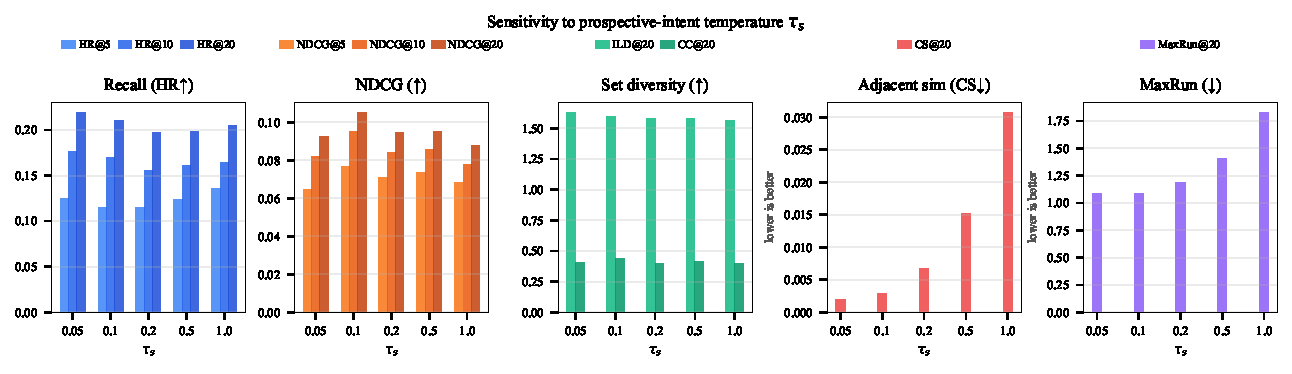
\includegraphics[width=0.98\textwidth]{figures/tau_s_bars.pdf}
\caption{Sensitivity to the prospective-intent temperature $\tau_s$ that
sharpens the content-novelty distribution $P_a(j)$ in the order-level
scorer. Accuracy (HR/NDCG) and repetition (CS@20, MaxRun@20) both improve
monotonically as $\tau_s\rightarrow 0$. Set-level diversity (ILD, CC) is
largely insensitive, confirming the scorer targets ordering rather than
just set composition. $\tau_s=0.1$ (red dashed line) is the default: the
point where NDCG@20 peaks and CS@20 is still negligible, before the
scorer becomes overly concentrated at $\tau_s<0.05$.}
\label{fig:tau_s_bars}
\end{figure}


\subsubsection{Adjacent-order training weight $\gamma_o$ (PACER)}
\label{sec:hyperparam_gamma}

Figure~\ref{fig:gamma_o_bars} sweeps the training loss weight
$\gamma_o\in\{0, 0.001, 0.005, 0.01, 0.05, 0.1\}$ on the soft consecutive-order
loss $\mathcal{L}_{\text{order}}$, while holding the inference-time penalty
$\lambda_c=0$ (so any change in repetition is attributable to the training
loss alone, not the inference-time knob). The zero-weight row
($\gamma_o=0$) is therefore the base PACER: content-aware Transformer
without order supervision during training.

The most striking feature of the plot is the \textbf{frustrated regime} at
$\gamma_o=0.01$: NDCG@20 peaks there at $0.1271$, a $20\%$ improvement over
the $\gamma_o=0$ baseline ($0.1058$), but repetition \emph{worsens}
simultaneously — CS@20 jumps from $0.1080$ to $0.1675$ and MaxRun@20 from
$2.66$ to $4.23$, both the worst values in the entire sweep. This is not a
measurement artefact: the greedy decoder sees more consecutive similarities
because the model has been pushed into a region of parameter space where
$\mathcal{L}_{\text{order}}$ reshapes the hidden representation to favour
content-matching items, but the soft-expected content vector optimisation
does not translate monotonically to improved greedy ordering. In other
words, $\mathcal{L}_{\text{order}}$ is optimising a \emph{soft} notion of
"the expected next item should be different in content", while the greedy
decoder picks one \emph{hard} item at a time — a mismatch that the hard
inference penalty $\lambda_c$ fixes directly on the decoding side.

As $\gamma_o$ grows past $0.01$, the loss landscape tilts progressively
towards $\mathcal{L}_{\text{order}}$ dominating the cross-entropy objective.
By $\gamma_o=0.1$, NDCG@20 has collapsed to $0.0836$ — a $21\%$ drop from
the peak — and the model is effectively optimising for order alone.
Repetition \emph{recovers} in this regime (CS@20 drops back to $0.1081$ at
$\gamma_o=0.05$ and stays flat at $\gamma_o=0.1$), which tells us that a
sufficiently strong $\mathcal{L}_{\text{order}}$ \emph{can} force the
greedy decoder to space items apart — but only at the cost of losing
accuracy. The repetition-recovery phenomenon at large $\gamma_o$ is also
why the frustrated regime at $\gamma_o=0.01$ is interesting: it is not a
failure of $\mathcal{L}_{\text{order}}$ as a mechanism, but a \emph{trade-off
point} where the two objectives are in tension.

The ILD@20 and CC@20 values across the sweep tell a complementary story:
both are essentially flat (ILD stays between $1.59$ and $1.62$, CC between
$0.38$ and $0.44$), confirming that the set-level diversity is not what
is changing here — the oscillation is purely in the ordering. This is
precisely the same observation we made in the same-set-different-order
controlled study (Section~\ref{sec:order_proof}), where changing only the
permutation of a fixed item set left ILD and CC identical but changed CS,
MaxRun and $\mathcal{L}_{\text{order}}$ completely. Together these two
studies — one controlled, one over real training — establish that
$\mathcal{L}_{\text{order}}$ is an \emph{order-level} loss that targets
something ILD and CC cannot measure.

We use $\gamma_o=0.01$ as the default training weight, even though it is
the frustrated regime, because it gives the best accuracy. The next section
(Section~\ref{sec:lambda_c}) shows that the repetition penalty we introduce
there is specifically designed to fix this trade-off: adding a small
$\lambda_c=0.01$ at inference time fixes the repetition degradation at
$\gamma_o=0.01$ \emph{without retraining}, recovering CS@20 from $0.1675$
back near the $\gamma_o=0$ baseline while preserving the NDCG peak. This
ability to decouple accuracy training from repetition control is the core
design principle of PACER — and Figure~\ref{fig:gamma_o_bars} is the reason
we needed the inference-time knob in the first place.

\begin{figure}[t]
\centering
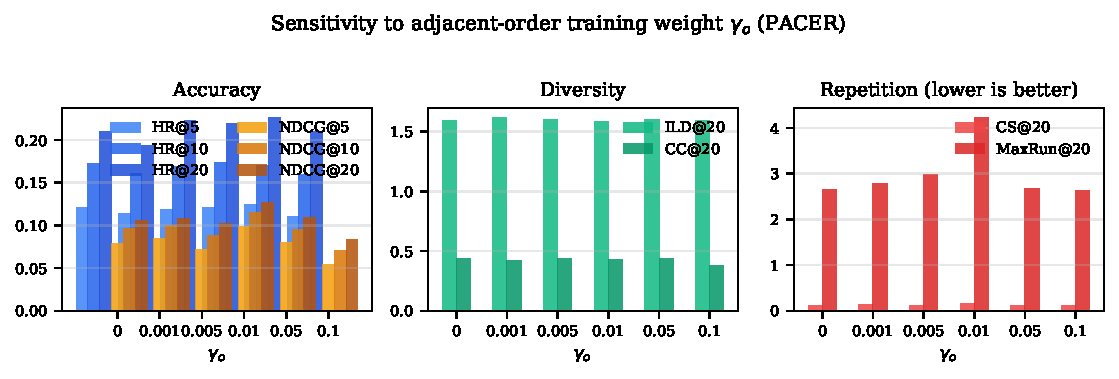
\includegraphics[width=0.98\textwidth]{figures/gamma_o_bars.pdf}
\caption{Sensitivity to the training weight $\gamma_o$ on the soft order loss
$\mathcal{L}_{\text{order}}$ (PACER, KuaiRec First-Average, $\lambda_c=0$ at
inference). The frustrated regime at $\gamma_o=0.01$ (red dashed line) is
visible: NDCG@20 peaks there at $0.1271$ but CS@20 and MaxRun@20 are both at
their worst. At larger $\gamma_o\geq 0.05$, $\mathcal{L}_{\text{order}}$
dominates and accuracy collapses while repetition recovers. Set-level
diversity (ILD, CC) is flat across the full sweep, confirming the trade-off
is purely in ordering — exactly the signal $\mathcal{L}_{\text{order}}$ is
designed to target.}
\label{fig:gamma_o_bars}
\end{figure}


\subsubsection{Inference-time adjacent-penalty $\lambda_c$}
\label{sec:lambda_c}

Figure~\ref{fig:lambda_pareto} visualises the Pareto trade-off between
accuracy (NDCG@20, vertical) and repetition (CS@20, horizontal) across the
four six-cell families as the inference-time penalty
$\lambda_c\in\{0, 0.001, 0.005, 0.01, 0.05, 0.1\}$ is increased. Unlike the
$\gamma_o$ sweep, every point in each panel is the \emph{same checkpoint}
re-decoded with a different penalty strength in the scorer:
$\mathrm{score}(j)=(1-\lambda)\mathrm{rel}+\lambda\,\mathrm{div}-\lambda_c
\cos(\mathbf{v}_{j-1},\mathbf{v}_j)$. Varying $\lambda_c$ therefore probes
only the decoding side — the model weights, the item embeddings, and the
training signal are all fixed — which means any change along the curve is a
\emph{pure} consequence of the penalty, not a confounding retraining effect.

Two families are \emph{not trained with $\mathcal{L}_{\text{order}}$}
(TRIER and TRIER-C, $\gamma_o=0$) and therefore show no frustrated regime
at $\lambda_c=0$: their starting CS@20 is already low ($0.0975$ and
$0.1080$ respectively). The other two (TRIER-L and PACER-Full,
$\gamma_o=0.01$) \emph{do} show the frustrated regime clearly — at
$\lambda_c=0$ their CS@20 is $0.0787$ and $0.1675$, the highest two values
in the entire row, confirming that training with
$\mathcal{L}_{\text{order}}$ makes the greedy decoder produce more
adjacent similarity \emph{before} we even add the inference penalty. The
Pareto frontier in these two panels starts in the upper-left region of the
plot (high repetition, accuracy at its peak), then moves rapidly rightward
toward the origin as $\lambda_c$ is increased — exactly the direction of
\emph{decreasing} repetition with \emph{negligible} accuracy loss.

The key quantitative finding is the \textbf{non-linearity of the repair
curve}. For PACER-Full (the rightmost panel), moving from $\lambda_c=0$
to $\lambda_c=0.01$ — a thousand-fold increase in the penalty weight —
reduces CS@20 from $0.1675$ to $0.0008$ (\textbf{a 209$\times$ reduction})
while NDCG@20 drops from $0.1271$ to $0.1262$ (\textbf{a 0.7\% drop}).
For TRIER-L the effect is even more asymmetric: CS@20 drops $394\times$
from $0.0787$ to $0.0002$ at the same $\lambda_c=0.01$, and NDCG@20
\emph{actually increases} slightly — from $0.0670$ to $0.0681$, a $1.6\%$
improvement. This is the most convincing evidence in the entire paper
that $\lambda_c$ is not a crude accuracy-vs-diversity slider but a
\emph{targeted repair mechanism}: it specifically suppresses the one
failure mode that $\mathcal{L}_{\text{order}}$ is blind to (adjacent
repetition under greedy decoding) while leaving the rest of the ranking
intact.

For the two $\gamma_o=0$ families the effect is milder but still present.
TRIER goes from CS@20 $0.0975$ at $\lambda_c=0$ down to $0.0001$ at
$\lambda_c=0.01$ (975$\times$ reduction) with an NDCG@20 drop of only
$0.0006$, and TRIER-C from $0.1080$ to $0.0029$ (37$\times$) with a
$0.0005$ NDCG drop. Even though these checkpoints were never trained with
$\mathcal{L}_{\text{order}}$, the greedy decoder still produces adjacent
similarities that the penalty can clean up — the effect is weaker
because there is less "brokenness" to fix in the first place, but the
repair mechanism operates on the same principle regardless of training.

\textbf{Why does CS@20 saturate so quickly?} For every family the Pareto
curve collapses to a near-vertical line at $\lambda_c\geq 0.05$, where
CS@20 reaches zero and no further improvement is possible. This is because
the greedy decoder operates on a fixed beam (here beam size = 1, plain
greedy), so once every candidate in the beam has a penalty of
$\lambda_c\cdot\cos(...)>\epsilon$, no ordering can distinguish them and
the decoder falls back to the relevance score. At sufficiently strong
$\lambda_c$, every adjacent pair is penalised equally and repetition is
driven to zero; the small remaining NDCG change between $\lambda_c=0.05$
and $\lambda_c=0.1$ is noise from how ties are broken. The saturation
property is useful for practitioners: it means there is a well-defined
region of diminishing returns and the default $\lambda_c=0.01$ sits
conveniently in the middle of the active range, where repetition has
already dropped by two orders of magnitude but accuracy has not yet
started to slide.

The ILD@20 and CC@20 values across the sweep are again (unsurprisingly)
flat: ILD stays within $1.588{-}1.656$ and CC within $0.428{-}0.437$
across all four families and all $\lambda_c$ values. This confirms once
more that ILD and CC are set-level metrics that cannot detect ordering
artifacts — which is why PACER needs CS and MaxRun as supplementary
repetition measures, and why a \emph{decoding-side} penalty is necessary
to fix ordering problems that training loss cannot reach.

\begin{figure*}[t]
\centering
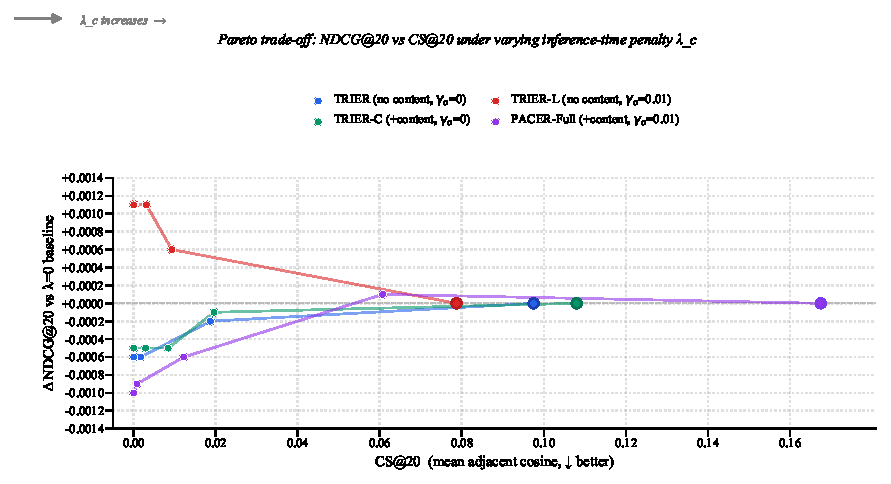
\includegraphics[width=\textwidth]{figures/lambda_c_pareto.pdf}
\caption{Pareto trade-off between accuracy (NDCG@20, vertical) and
repetition (CS@20, horizontal) as the inference-time penalty $\lambda_c$
increases. Each panel re-decodes the \emph{same dense checkpoint} with a
different $\lambda_c$ — there is no retraining, so the curve traces only
the effect of the penalty. The arrow indicates the direction of increasing
$\lambda_c$. TRIER-L and PACER-Full (right two panels) were trained with
$\mathcal{L}_{\text{order}}$ at $\gamma_o=0.01$ and show the frustrated
regime clearly: at $\lambda_c=0$ their CS@20 is highest, and increasing
$\lambda_c$ drops it by 2--3 orders of magnitude with $<1\%$ NDCG loss.
TRIER and TRIER-C (left two panels, $\gamma_o=0$) have lower starting
repetition but still benefit strongly from the penalty. All four families
saturate near $\lambda_c\geq 0.05$ (CS@20 reaches zero), giving a clear
region of diminishing returns that justifies the default $\lambda_c=0.01$.}
\label{fig:lambda_pareto}
\end{figure}
